\documentclass[11pt]{article}
\usepackage{amsmath, amssymb, amsthm,enumerate}
\usepackage{color}
\usepackage{tikz}
\usetikzlibrary{calc}
\usetikzlibrary{math}
\usetikzlibrary{patterns}
\usetikzlibrary{decorations.pathreplacing}
\usepackage{amssymb}

\begin{document}

		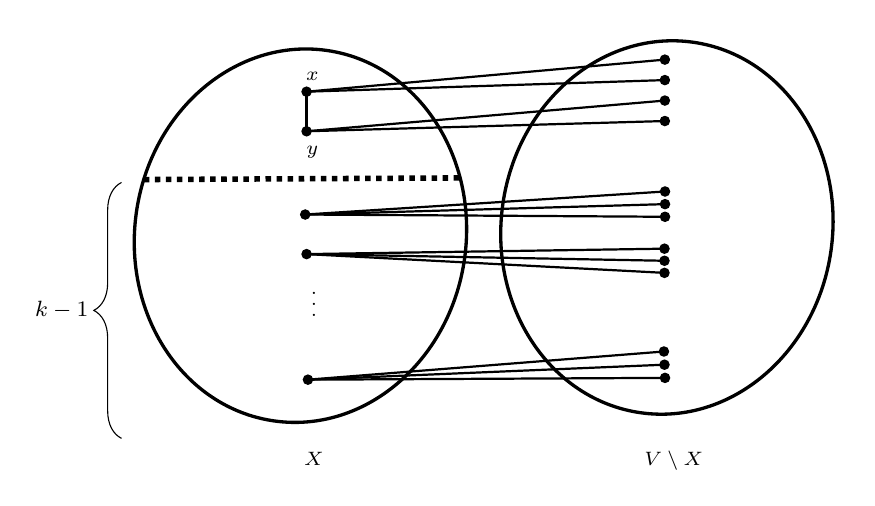
\begin{tikzpicture}[scale=1.3]
\draw [rotate around={81.8698976458454:(-1.56,3.48)},line width=1.2pt] (-1.56,3.48) ellipse (1.82786947059178cm and 1.6189832616557454cm);
\draw [rotate around={81.86989764584541:(2.02,3.56)},line width=1.2pt] (2.02,3.56) ellipse (1.8278694705917768cm and 1.6189832616557427cm);
\draw [line width=2.pt,dotted] (-3.090847313658136,4.028220675271917)-- (0.,4.044208981538004);
\draw [line width=0.8pt] (-1.5,4.886666666666666)-- (2.,5.2);
\draw [line width=0.8pt] (-1.5,4.886666666666666)-- (2.,5.);
\draw [line width=0.8pt] (-1.5,4.5)-- (2.,4.8);
\draw [line width=0.8pt] (-1.5,4.5)-- (2.,4.6);
\draw [line width=0.8pt] (-1.5133333333333343,3.686666666666666)-- (2.001672135052165,3.9117106151847634);
\draw [line width=0.8pt] (-1.5133333333333343,3.686666666666666)-- (2.001672135052165,3.7881638705323435);
\draw [line width=0.8pt] (-1.5,3.3)-- (1.9963005374585814,3.2348893183932463);
\draw [line width=0.8pt] (-1.5,3.3)-- (1.9963005374585814,3.11671417133441);
\draw [line width=0.8pt] (-1.5,4.886666666666666)-- (-1.5,4.5);
\draw [line width=0.8pt] (-1.4866666666666677,2.073333333333333)-- (1.990928939864998,2.3485757154519744);
\draw [line width=0.8pt] (-1.4866666666666677,2.073333333333333)-- (1.9963005374585814,2.2196573732059712);
\draw [line width=0.8pt] (-1.5133333333333343,3.686666666666666)-- (2.001672135052165,3.664617125879924);
\draw [line width=0.8pt] (-1.5,3.3)-- (1.9963005374585814,3.353064465452083);
\draw [line width=0.8pt] (-1.4866666666666677,2.073333333333333)-- (2.001672135052165,2.090739030959968);
\begin{scriptsize}
\draw [fill=black] (-1.5,4.886666666666666) circle (1.3pt);
\draw[color=black] (-1.4442688823907668,5.041287969232268) node {$x$};
\draw [fill=black] (-1.5,4.5) circle (1.3pt);
\draw[color=black] (-1.4442688823907668,4.3) node {$y$};
\draw [fill=black] (-1.5133333333333343,3.686666666666666) circle (1.3pt);
\draw [fill=black] (-1.5,3.3) circle (1.3pt);
\draw[color=black] (-1.4271668350085396,2.8864299990716606) node {$\vdots$};
\draw [fill=black] (-1.4866666666666677,2.073333333333333) circle (1.3pt);
\draw [fill=black] (2.,5.2) circle (1.3pt);
\draw [fill=black] (2.,5.) circle (1.3pt);
\draw [fill=black] (2.,4.8) circle (1.3pt);
\draw [fill=black] (2.,4.6) circle (1.3pt);
\draw [fill=black] (2.001672135052165,3.9117106151847634) circle (1.3pt);
\draw [fill=black] (2.001672135052165,3.7881638705323435) circle (1.3pt);
\draw [fill=black] (1.9963005374585814,3.2348893183932463) circle (1.3pt);
\draw [fill=black] (1.9963005374585814,3.11671417133441) circle (1.3pt);
\draw [fill=black] (1.990928939864998,2.3485757154519744) circle (1.3pt);
\draw [fill=black] (1.9963005374585814,2.2196573732059712) circle (1.3pt);

\draw[color=black] (-1.4271668350085396,1.2959395925245456) node {$X$};
\draw[color=black] (2.087303902039137,1.2788375451423184) node {$V\setminus X$};
\draw [fill=black] (2.001672135052165,3.664617125879924) circle (1.3pt);
\draw [fill=black] (1.9963005374585814,3.353064465452083) circle (1.3pt);
\draw [fill=black] (2.001672135052165,2.090739030959968) circle (1.3pt);
\draw [decorate,decoration={brace,amplitude=10pt,mirror,raise=4pt},yshift=0pt] (-3.2,4) -- (-3.2,1.5)  node [black,midway,xshift=-0.9cm] {\footnotesize $k-1$};
\end{scriptsize}
\end{tikzpicture}

\end{document}